% Created 2024-04-09 Tue 21:29
% Intended LaTeX compiler: pdflatex
\documentclass[presentation]{beamer}
\usepackage[utf8]{inputenc}
\usepackage[T1]{fontenc}
\usepackage{graphicx}
\usepackage{longtable}
\usepackage{wrapfig}
\usepackage{rotating}
\usepackage[normalem]{ulem}
\usepackage{amsmath}
\usepackage{amssymb}
\usepackage{capt-of}
\usepackage{hyperref}
\mode<beamer>{\usetheme{Madrid}}
\definecolor{SUred}{rgb}{0.59375, 0, 0.17969} % SU red (primary)
\definecolor{SUblue}{rgb}{0, 0.17578, 0.38281} % SU blue (secondary)
\setbeamercolor{palette primary}{bg=SUred,fg=white}
\setbeamercolor{palette secondary}{bg=SUblue,fg=white}
\setbeamercolor{palette tertiary}{bg=SUblue,fg=white}
\setbeamercolor{palette quaternary}{bg=SUblue,fg=white}
\setbeamercolor{structure}{fg=SUblue} % itemize, enumerate, etc
\setbeamercolor{section in toc}{fg=SUblue} % TOC sections
% Override palette coloring with secondary
\setbeamercolor{subsection in head/foot}{bg=SUblue,fg=white}
\setbeamercolor{date in head/foot}{bg=SUblue,fg=white}
\institute[SU]{Shenandoah University}
\titlegraphic{\includegraphics[width=0.5\textwidth]{\string~/Documents/suLogo/suLogo.pdf}}
\newcommand{\R}{\mathbb{R}}
\usepackage{tikz}
\usepackage{pgfplots}
\usetheme{default}
\author{Chase Mathison\thanks{cmathiso@su.edu}}
\date{10 April 2024}
\title{The Law of Cosines}
\hypersetup{
 pdfauthor={Chase Mathison},
 pdftitle={The Law of Cosines},
 pdfkeywords={},
 pdfsubject={},
 pdfcreator={Emacs 29.1 (Org mode 9.6.7)}, 
 pdflang={English}}
\begin{document}

\maketitle

\section{Announcements}
\label{sec:org52ab2c0}
\begin{frame}[label={sec:org15bca4f}]{Announcements}
\begin{enumerate}
\item Homework in M.O.M.
\item Project in M.O.M.
\item Office hours 10am - 11am
\end{enumerate}
\end{frame}

\section{Lecture}
\label{sec:org2d1f5ab}
\begin{frame}[label={sec:orgd6e304f}]{The Law of Cosines}
Now, let's develop another very special law, the Law of Cosines.

\begin{center}
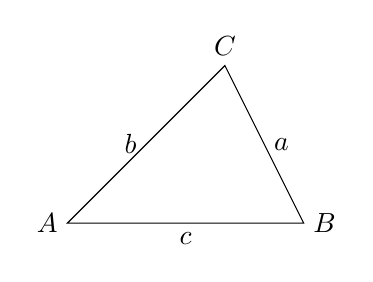
\begin{tikzpicture}[scale=1]
  \node[left] at (0,0) {$A$};
  \node[right] at (3,0) {$B$};
  \node[above] at (2,2) {$C$};
  \draw (0,0) -- node[below] {$c$} (3,0) -- node[right] {$a$} (2,2) -- node[left] {$b$} cycle;
\end{tikzpicture}
\end{center}

\vspace{10in}
\end{frame}

\begin{frame}[label={sec:org4c169b7}]{The Law of Cosines}
\end{frame}

\begin{frame}[label={sec:org9739c74}]{The Law of Cosines}
We've just developed the Law of Cosines!

\begin{block}{The Law of Cosines}
For any triangle with angles \(A,B\) and \(C\) and corresponding side lengths \(a,b\) and \(c\), we have

\[
a^2 = \hspace{2in}\]
\[
b^2 = \hspace{2in}\]
\[
c^2 = \hspace{2in}\]
\end{block}
\end{frame}

\begin{frame}[label={sec:org0f14db2}]{Using the Law of Cosines}
In practice, we need to use the Law of Cosines to solve an oblique
triangle in which we know two side lengths and the angle included
between those sides: \uline{\hspace*{1in}}.

Here's an example:

\begin{center}
  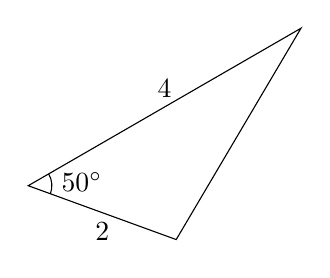
\begin{tikzpicture}
    \draw (-20:2) -- node[below] {2} (0,0) -- node[above] {4} (30:4) -- cycle;
    \draw (-20:0.3) arc (-20:30:0.3);
    \node[right] at (0.3,0.05) {$50^\circ$};
  \end{tikzpicture}
\end{center}
\end{frame}


\begin{frame}[label={sec:orgdace2d7}]{Example}
\end{frame}

\begin{frame}[label={sec:orge255af3}]{Example}
We can also use the law of Cosines if we know all of the sides of an
oblique triangle, but none of the angles:

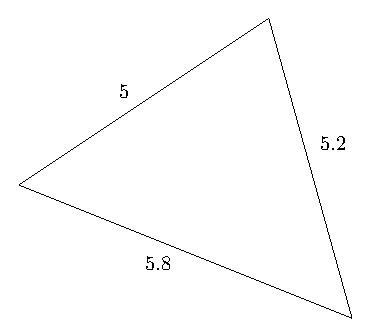
\includegraphics[width=0.4\textwidth]{./sss}
\vspace{10in}
\end{frame}

\begin{frame}[label={sec:org7b62172}]{Applied Example}
Let's finish up that last example:

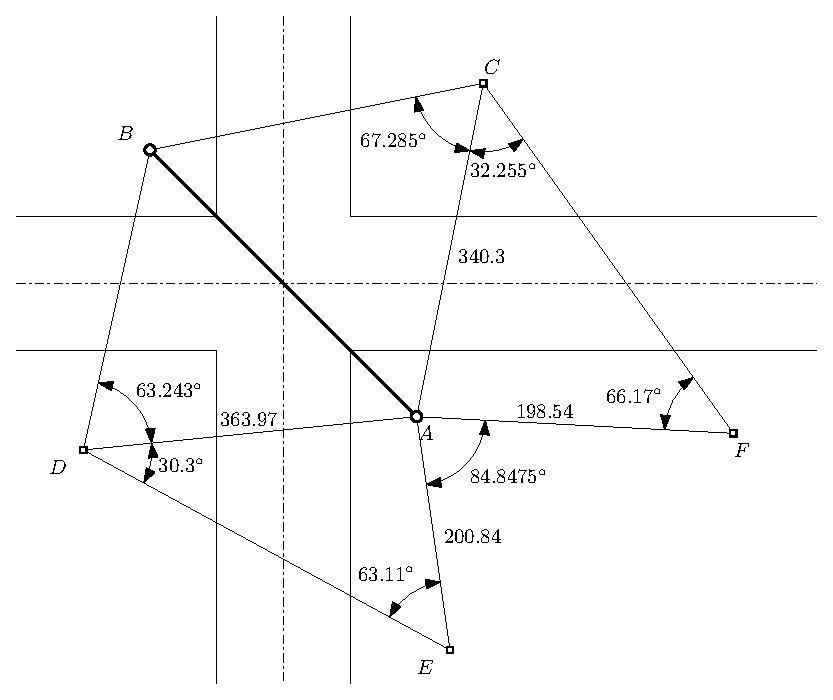
\includegraphics[width=0.5\textwidth]{./trigStar}
\vspace{10in}
\end{frame}
\end{document}